\documentclass{bioinfo}
\copyrightyear{2015} \pubyear{2015}

%\usepackage[top=1.3in, bottom=1.3in, left=1in, right=1in]{geometry}
\usepackage{floatrow}
\usepackage{graphicx} % more modern
\usepackage{amssymb}
\usepackage{amsmath}
\usepackage{booktabs}
\usepackage{subfigure} 
\usepackage{natbib}
%\usepackage[footnotesize]{caption}
\usepackage{multirow}
\usepackage{url}

%%%%%%%%%%%%%%%%%%%%%%%%%%

\newfloatcommand{capbtabbox}{table}[][11cm]
\newcommand{\argmin}{\operatornamewithlimits{argmin}}

%%%%%%%%%%%%%%%%%%%%%%%%%%
%\setcounter{tocdepth}{3}
%\setcounter{secnumdepth}{0}
%%%%%%%%%%%%%%%%%%%%%%%%%%


\access{Advance Access Publication Date: Day Month Year}
\appnotes{Manuscript Category}

\begin{document}
\firstpage{1}

\subtitle{Subject Section}

\title[Multitask matrix completion]{Multitask matrix completion for learning protein interactions across diseases}

\author[Kshirsagar \textit{et~al}.]{Meghana Kshirsagar$^{1}$, Keerthiram Murugesan$^{2}$, Jaime G. Carbonell$^{2}$ and Judith Klein-Seetharaman$^{3}$}
\address{$^{1}$Memorial Sloan Kettering Cancer Center, 1275 York Ave., NY 10021\\
$^{2}$Language Technologies Institute, Carnegie Mellon Univ., 5000 Forbes Ave., Pittsburgh PA 15213, USA\\
$^{3}$Metabolic \& Vascular Health, Warwick Medical School, Univ. of Warwick, Coventry, UK
}

\corresp{$^\ast$To whom correspondence should be addressed.}

\history{Received on XXXXX; revised on XXXXX; accepted on XXXXX}

\editor{Associate Editor: XXXXXXX}

\abstract{\textbf{Motivation:}
Disease causing pathogens such as viruses, introduce their proteins into the host cells 
where they interact with the host's proteins enabling the virus to replicate inside the host.
These interactions between pathogen and host proteins are key to understanding infectious diseases.
Often multiple diseases involve phylogenetically related or biologically similar pathogens. Here we present a multitask learning method to jointly model interactions between human proteins and three different, but related viruses: \textit{Hepatitis C}, \textit{Ebola} virus and \textit{Influenza A}. \\
\textbf{Results:}
Our multitask matrix completion based model uses a shared low-rank structure in addition to a task-specific sparse structure to incorporate the various interactions.
We obtain between 7 to 39 percentage points improvement in predictive performance over prior state-of-the-art models. 
We show how our model's parameters can be interpreted to reveal both general and specific
interaction-relevant characteristics of the viruses. \\
\textbf{Availability:}
Code and data is available at: \url{http://www.cs.cmu.edu/~mkshirsa/bsl_mtl.tgz}\\
\textbf{Contact:}
\href{mkshirsa@cs.cmu.edu}{mkshirsa@cs.cmu.edu}
}

\maketitle

%\begin{abstract}
%\section{Motivation}
%Disease causing pathogens such as viruses, introduce their proteins into the host cells 
%where they interact with the host's proteins enabling the virus to replicate inside the host.
%These interactions between pathogen and host proteins are key to understanding infectious diseases.
%Often multiple diseases involve phylogenetically related or biologically similar pathogens. Here we present a multitask learning method to jointly model interactions between human proteins and three different, but related viruses: \textit{Hepatitis C}, \textit{Ebola} virus and \textit{Influenza A}. 
%\section{Results}
%Our multitask matrix completion based model uses a shared low-rank structure in addition to a task-specific sparse structure to incorporate the various interactions.
%We obtain between 7 to 39 percentage points improvement in predictive performance over prior state-of-the-art models. 
%We show how our model's parameters can be interpreted to reveal both general and specific
%interaction-relevant characteristics of the viruses. \\
%\section{Availability}
%Our code and data is available at: \url{http://www.cs.cmu.edu/~mkshirsa/bsl_mtl.tgz}\\
%\section{Contact}
%\href{mkshirsa@cs.cmu.edu}{mkshirsa@cs.cmu.edu}
%\end{abstract}


\section{Introduction}


Infectious diseases such as H1N1 influenza, the recent Ebola outbreak and bacterial infections, such as the recurrent \textit{Salmonella} and \textit{E. coli} outbreaks
are a major health concern worldwide, causing millions of illnesses and many deaths each year. 
Key to the infection process are host-pathogen interactions at the molecular level, where pathogen proteins physically bind to human proteins
to manipulate important biological processes in the host cell, to evade the host's immune response and to multiply within the host.
Very little is known about these protein-protein interactions (PPIs) between pathogen and host proteins for any individual disease.
However, such PPI data is widely available across several diseases, and the central question in this
paper is: \emph{Can we model host-pathogen PPIs better by leveraging
data across multiple diseases?} This is of particular interest for 
lesser known or recently evolved diseases where the data is particularly scarce. Furthermore, it
allows us to learn models that generalize better across diseases by
modeling global phenomena related to infection.

An elegant way to formulate the interaction prediction problem is via a graph completion based framework, where we have several bipartite 
graphs over multiple hosts and pathogens. % as illustrated in Figure \ref{fig:hpppigraph}.
Nodes in the graphs represent host proteins (circles) and pathogen proteins (triangles), with edges between them representing interactions 
(host protein $\frac{interacts}{}$ pathogen protein).
Given some observed edges (interactions obtained from laboratory based experiments), we wish to predict the other edges in the graphs.
Such bipartite graphs arise in a plethora of problems including: recommendation systems (user $\frac{prefers}{}$ movie), 
citation networks (author $\frac{cites}{}$ paper), disease-gene networks (gene $\frac{influences}{}$ disease) etc. 
In our problem, each bipartite graph $\mathcal{G}$ can be represented using a matrix $M$, where the rows correspond to pathogen proteins 
and columns correspond to host proteins.
The matrix entry $M_{ij}$ encodes the edge between pathogen protein $i$ and host protein $j$ from the graph, with $M_{ij}=1$ for the observed interactions. 
Thus, the graph completion problem can be mathematically modeled as a matrix completion problem \citep{candes08}. 
%Traditional approaches towards matrix completion rely on the assumption that the underlying function that generated the matrix can be decomposed into a small number of `latent' factors. The solution based on this assumption involves finding a low-rank matrix factorization for $M$, mathematically expressed as: finding $U$ and $V$ such that $M \approx UV^T$. Here the parameters $U$ and $V$ are called the factor matrices and represent the latent properties of the host and pathogen proteins respectively. In the recommendation systems example, the `low rank' structure suggests that movies can be grouped into a small number of latent `genres'. In the case of proteins these latent properties could correspond to various \textit{biological functions} of proteins or encode \textit{interaction propensities}.

Most of the prior work on host-pathogen PPI prediction has modeled each bipartite graph separately, and hence cannot exploit the similarities 
in the edges across the various graphs. Here we present a \textit{multitask} matrix completion method that \textit{jointly models} 
several bipartite graphs by sharing information across them. 
From the multitask perspective, a \textit{task} is the graph between one host and one pathogen (can also be seen as interactions relevant to one disease). 
We focus on the setting where we have a single host species (human) and several related viruses, where we hope to gain from the 
fact that similar viruses will have similar strategies to infect and hijack biological processes in the human body.
Such opportunities for sharing arise in other applications as well: for instance, predicting user preferences in movies may inform preferences in selection of books, 
or vice-versa, as movies and books are semantically related. Multitask learning based models that incorporate and exploit these correlations should benefit from 
the additional information.% and result in a better prediction performance. 

Our multitask matrix completion based model is motivated by the following biological intuition governing protein interactions across diseases.
\begin{enumerate}
\item An interaction depends on the structural properties of the proteins, which are conserved across similar viruses as they have evolved from common ancestors. Our model thus needs a component to capture these latent similarities, which is \textit{shared} across tasks.
%This latent structural similarity can be expressed via latent factors that project the proteins into a shared lower dimensional subspace that is common to all tasks.
\item In addition to the shared properties discussed above, each pathogen has also evolved specialized mechanisms to target host proteins. These are unique to the pathogen and can be expressed using a \textit{task-specific} parameter in the model.
\end{enumerate}

This leads us to the following model that incorporates the above ideas. The interactions matrix $M_t$ of task $t$ can be written as: $M_t = \mu_t *\; \textrm{(shared component)} + (1-\mu_t) *\; \textrm{(specific component)} $, with hyperparameter $\mu_t$ allowing each task to customize its amount of shared and specific components.



To incorporate the above ideas, we assume that the interactions matrix $M$ is generated from two components. 
The first component has low-rank latent factors over the human and virus proteins,
with these latent factors jointly learned over all tasks. The second component involves a task specific parameter, on which we
additionally impose a sparsity constraint as we do not want this parameter to overfit the data. Section~\ref{ourmodel} discusses
our model in detail. We trade-off the relative importance of the two components using task-specific hyperparameters.
Our model can thus learn what is conserved and what is different across pathogens, rather than having to specify it manually. 

The key challenges in inducing such a model are: (1) In addition to the interactions from each graph, it should exploit information available in the form of features. 
(2) Exploiting features is particularly crucial since the graph $\mathcal{G}$ is often extremely sparse, i.e there are a large number of nodes and very few edges are observed. 
There will be proteins (i.e nodes) that are not involved in any known interactions -- called the \textit{cold start problem} in the recommendation systems community. 
The model should be able to predict the existence of links (or their absence) between such prior `unseen' node pairs. 
This is of particular significance in graphs that capture biological phenomena. For instance, the host-pathogen PPI network
of human-Ebola virus (column-3, Table \ref{datasets}) has $\approx$ 90 observed edges (equivalent to 0.06\% of the possible edges) which involve only 2 distinct virus proteins. 
(3) A side-effect of having scarce data is the availability of a large number of unlabeled examples, 
i.e pairs of nodes with no edge between them. 
These unlabeled examples can contain information about the graph as a whole, and a good model should be able to use them.
%(4) ---- class skew ----

The main contributions of this work are:
\begin{itemize}
\item We extend a prior matrix completion model \citep{abernethy} to the multitask setting. This extension is new.
\item Unlike most prior approaches, our model exploits node-based features which allows us to deal with the `cold start' problem (generating predictions on unseen nodes).
\item We apply the model to an important, real-world problem -- prediction of interactions in disease-relevant host-pathogen protein networks, for multiple related diseases. We demonstrate the superior performance of our model over prior state-of-the-art multitask models.
\item We use unlabeled data to initialize the parameters of our model, which serves as a prior. This gives us a modest boost in prediction performance.
\end{itemize}

\subsection{Background: Host-pathogen protein interactions}
%An important part of our sustenance depends on how we counter infectious diseases -- those that are caused by external agents like pathogens. To understand how these microbial organisms reside and disrupt the host processes we need to comprehend the cross-organism protein interactions between the host species such as mammals, and the causative pathogen species such as viruses and bacteria. %These interactions  pathogen proteins physically bind with human proteins to manipulate important biological processes in the host cell, evade the host immune response and multiply within the host. 
The experimental discovery of host-pathogen protein interactions involves biochemical and biophysical methods such as co-immunoprecipitation (co-IP), yeast two-hybrid (Y2H) assays, co-crystalization. The host-pathogen protein interactions from several small-scale and high throughput experiments are aggregated by databases such as MINT \citep{virusmint}, HPIDB \citep{hpidb}, PHISTO \citep{phisto} etc by literature curation. These databases are valuable sources of information to bioinformaticians for developing models. \\

\noindent\textbf{Prediction of host-pathogen PPIs}: The most reliable experimental methods for studying protein-protein interactions (PPI) are often very time-consuming and expensive, making it hard to investigate the prohibitively large set of possible host-pathogen interactions -- for example, the bacterium \textit{Bacillus anthracis} which causes anthrax has about 2321 proteins which when coupled with the 100,000 or so human proteins gives $\approx$232 million protein pairs to test, experimentally. Computational techniques complement laboratory-based methods by predicting highly probable PPIs. These techniques use the known interactions data from previous experiments and predict the most plausible new interactions. In particular, supervised machine learning based methods use the few known interactions as training data and formulate the interaction prediction problem in a classification setting, with target classes: ``interacting'' or ``non-interacting''. Features are derived using various attributes of the two proteins such as: protein sequences from UniProt \citep{UniProt}, protein structure from PDB, gene ontology from GO database \citep{GO}.

\subsection{Prior work}
%\label{prior_work}
Most of the prior work in PPI prediction has focussed on building models separately for individual 
organisms \citep{chen,yeast,struct2net,qi06} or on building a model specific to a disease in the case of host-pathogen PPI 
prediction \citep{tastan09,qi09,dyer07,me12}. There has been little work on combining PPI datasets with the goal of improving 
prediction performance for multiple organisms. \cite{qi2010} proposed a semi-supervised multi-task framework to predict PPIs from partially labeled reference sets. \cite{me_ismb_2013} develop a task regularization based
framework called MTPL that incorporates the similarity in biological pathways targeted by various diseases to 
couple multiple tasks together. Matrix factorization based protein-protein interaction (PPI) prediction has seen very little work, mainly due to the extremely sparse nature of these datasets which makes it very difficult to get reliable predictors. \cite{ppi_cmf} use a CMF-based approach in a multi-task learning setting for within species PPI prediction. The methods used 
in all prior work on PPI prediction do not explicitly model the features of the proteins and cannot be applied on proteins which have no known interactions available. Our work addresses both these issues.
%in using a formulation of the matrix completion problem originally proposed in the work by \cite{abernethy}.

A majority of the prior work in the relevant areas of collaborative filtering and link prediction includes single relation models that use neighbourhood based prediction \citep{sarwar01}, matrix factorization based approaches \citep{koren09,menon_ecml11} and bayesian approaches using graphical models \citep{jin02,phung09}. 
%The matrix factorization based methods have been more popular than the other methods. 
There have also been multitask approaches on link prediction \citep{zhang12,cao_icml2010,li09,cmf} however many of those models do not incorporate features of the nodes in the graph. 
%\cite{li11} presents a survey on multitask/transfer methods in collaborative filtering. 
%The multi-relational learning literature \cite{xu09} and the work on link prediction in heterogenous networks is not relevant as their setting involves \textit{different types of relationships} between the \textit{same} set of nodes.
%The prior work on incorporating side information in the form of features of the nodes (users/movies) and edges
%has been proposed for single-graph link prediction problems. 
\cite{menon_ecml11} combine linear 
and bilinear features, latent parameters on the nodes and several other parameters into a function that minimizes a ranking loss for link prediction in a single graph. 
%Probabilistic models to combine network structure with node features have also been proposed. 
\cite{abernethy} cast the problem of matrix completion in terms of the abstract problem of learning linear operators. Their framework allows the incorporation of features and kernels. We extend their bilinear model for the multitask setting. There has been a lot of work on other low-rank models for multitask learning \citep{ando2005,ji2009,chen2012,chen2013}. % that try to capture the task relationship via a shared low-rank structure over the model parameters. Chen et al \cite{chen2012} have developed efficient algorithms for sparse and low-rank multitask learning models for classification. 
Another related line of work is co-embedding, where the goal is to embed different types of objects in the same shared lower-dimensional space \citep{mirzazadeh:2015}.

%\subsection{Background: Host-pathogen protein interactions}
%The biochemical and biophysical methods that study protein-protein interactions (PPI) are very time-consuming and expensive, making it hard to investigate the 
%prohibitively large set of possible host-pathogen interactions\footnote{The bacterium \textit{Bacillus anthracis} which causes anthrax has $\approx$ 2321 proteins, the human body has $\approx$ 100,000 giving $\approx$232 million protein pairs to test}. 
%Computational techniques complement these laboratory-based methods by predicting probable PPIs allowing biologists to focus their resources and time on the more promising candidates. Supervised learning methods use the few experimentally-discovered interactions as training data and solve the problem in a classification setting, with classes: ``interacting'' or ``non-interacting''. These use features derived using protein properties such as: protein sequences, protein structure, gene function etc.

%\noindent{\textbf{Multi-task learning for host-pathogen PPI prediction}}: Pathogens that have similar DNA sequences produce proteins with similar functions and will have similar strategies of infecting their hosts. Knowledge can thus be shared across diseases to better understand various global phenomena related to infection and to improve predictive models. Multitask approaches thus have several advantages, especially in dealing with data scarcity issues that hamper the construction of disease-specific models for less studied diseases. In our setting, each disease can be considered as a `task' i.e the PPIs involving the host and the causative pathogen. Figure \ref{fig:hpppigraph} shows the various possible multitask settings for this problem.


\section{Bilinear low-rank matrix decomposition}
In this section, we present the matrix decomposition model that we extend for the multitask scenario. In the context of our problem, at a high level, this model states that -- protein interactions can be 
expressed as dot products of features in a lower dimensional subspace.

\label{MCintro}
Let $\mathcal{G}_{t}$ be a bipartite graph connecting nodes of type $\upsilon$ with nodes of type $\varsigma$. Let there be $m_t$ nodes of type $\upsilon$ and $n_t$ nodes of type $\varsigma$. We denote by $M \in \mathbb{R}^{m_t \times n_t}$, the matrix representing the edges in $\mathcal{G}_{t}$. Let the set of observed edges be $\Omega$. 
Let $\mathcal{X}$ and $\mathcal{Y}$ be the feature spaces for the node types $\upsilon$ and $\varsigma$ respectively. For the sake of notational convenience we assume that the two feature spaces have the same dimension $d_t$ \footnote{the dimensions being different does not influence the method or the optimization in any way}. Let $\mathbf{x}_i \in \mathcal{X}$ denote the feature vector for a node $i$ of type $\upsilon$ and $\mathbf{y}_j \in \mathcal{Y}$ be the feature vector for node $j$ of type $\varsigma$. The goal of the general matrix completion problem is to learn a function $f : \mathcal{X} \times \mathcal{Y} \rightarrow \mathbb{R}$ that also explains the observed entries in the matrix $M$. We assume that the function $f$ is bilinear on $\mathcal{X} \times \mathcal{Y}$. This bilinear form was first introduced by \cite{abernethy} and takes the following form:
\begin{equation}
f(\mathbf{x}_i, \mathbf{y}_j) = \mathbf{x}_i^\intercal H \mathbf{y}_j = \mathbf{x}_i^\intercal U V^\intercal \mathbf{y}_j
\end{equation}

The factor $H \in \mathbb{R}^{d_t \times d_t}$ maps the two feature spaces $\mathcal{X}$ and $\mathcal{Y}$. This model assumes that $H$ has a low-rank factorization given by $H = U V^\intercal$, where $U \in \mathbb{R}^{d_t \times k}$ and $V \in \mathbb{R}^{d_t \times k}$. The factors $U$ and $V$ project the two feature spaces to a common lower-dimensional subspace of dimension $k$. While the dimensionality of the feature spaces $\mathcal{X}$ and $\mathcal{Y}$ may be very large, the latent lower dimensional subspace is sufficient to capture all the information pertinent to interactions. To predict whether two new nodes (i.e nodes with no observed edges) with features $\mathbf{p}_i$ and $\mathbf{q}_j$ interact, we simply need to compute the product: $\mathbf{p}_i U V^\intercal \mathbf{q}_j$. This enables the model to avoid the cold start problem that many prior models suffer from. The objective function to learn the parameters of this model has two main terms: (1) a data-fitting term, which imposes a penalty for deviating from the observed entries in $\Omega$ and (2) a low-rank enforcing term on the matrix $H$. 

The first term can be any loss function such as squared error, logistic-loss, hinge loss. We tried both squared error and logistic-loss and found the performance to be similar. The squared error function has the advantage of being amenable to adaptive step-size based optimization which results in a much faster convergence. The low-rank constraint on $H$ (mentioned in (2) above) is NP-hard to solve and it is standard practice to replace it with either the trace-norm or the nuclear norm. Minimizing the trace norm (i.e. sum of singular values) of $H = UV^\intercal$, is equivalent to minimizing $\|U\|^2_F + \|V\|^2_F$. This choice makes the overall function easier to optimize:
\begin{equation}
\label{objective}
\begin{array}{ll}
\mathcal{L}(U,V) & =\displaystyle{\sum_{(i,j) \in \Omega}} c_{ij} \; \ell(M_{ij}, \mathbf{x}_i^\intercal U V^\intercal \mathbf{y}_j) + \lambda ( \|U\|^2_F + \|V\|^2_F ) \\
& \textrm{ where } \ell(a, b) = (a - b)^2
\end{array}
\end{equation}

The constant $c_{ij}$ is the weight/cost associated with the edge $(i,j)$ which allows us to penalize the error on individual instances independently. The parameter $\lambda$ controls the trade-off between the loss term and the regularizer. 
%The function in equation(\ref{objective}) is non-convex. To optimize this function a common procedure called alternating minimization (AltMin) is used, which fixes one of the two parameters and optimizes w.r.t the other. 


%\noindent\textbf{Biological intuition}: The projection allows each feature to take on several different weights and hence allows for more flexibility as compared to a linear model. In the context of the host-pathogen PPI prediction, one can interpret this new subspace to represent latent biological characteristics of the features or binding propensities. In the Results section, we will analyze these parameters $U$ and $V$ and show how they can be used to understand the PPIs data better.

\begin{figure*}
\begin{floatrow}
\capbtabbox[0.68\textwidth]{%
\begin{footnotesize}
\begin{tabular}{c|r|r|r} 
\hline
Task $\rightarrow$ &{\textit{Influenza A} } &\textit{Hepatitis C} & {\textit{Ebola}}\\
& (28 strains) & (5 strains, many isolates)  & (3 strains) \\
number of HP PPIs (positives) & 848 & 981 & 90 \\\hline
number of non-homologous PPIs & 274 & 270 & 75 \\ \hline
\# of unique virus proteins in dataset & 54 & 151 & 2 \\\hline
\# of unique human proteins in dataset & 362 & 385 & 88 \\\hline
total \# of virus proteins in & 542 & 163 & 38 \\
UniProtKB across strains $^\dagger$ & & & \\ \hline
number of negatives & 84800 & 98100 & 9000 \\\hline
density of observed graph$^\ddagger$ (as \%) & .15 & .60 & .20 \\\hline
\multicolumn{4}{l}{\scriptsize{HP PPI: host-pathogen protein protein interactions}}\\
\multicolumn{4}{l}{\scriptsize{$\ddagger$ Density = (no. of positives + no. of negatives)/ total number of possible edges. The denominator was computed }} \\
\multicolumn{4}{l}{\scriptsize{\hspace{0.1cm} considering all proteins from all strains of the virus and $\approx$ 100,000 human proteins.}}\\
\multicolumn{4}{l}{\scriptsize{$\dagger$ this is the number of `reviewed' proteins on UniProtKB from all strains in our data}} \\ \hline
\end{tabular}
\end{footnotesize}
}
{
\caption{Tasks and their sizes (a column corresponds to one bipartite graph between human proteins and the virus indicated in the column header). More importantly, each task represents several strains of one virus species. We pool together PPI from all strains as the number of interactions per strain is very small and not representative. PPI data from different strains often involves homologous proteins (virus proteins or/and human proteins) as these were curated from different publications/studies involving the virus. The second row gives a conservative estimate of the number of non-homologous PPI. These were obtained by computing BLAST sequence similarity (see Section \ref{sec:phisto} for details). All pathogens are single stranded RNA viruses. The last row shows that each of our graphs is extremely sparse.} 
\label{datasets}
}
\ffigbox[0.28\textwidth]{%
%trim option's parameter order: left bottom right top
%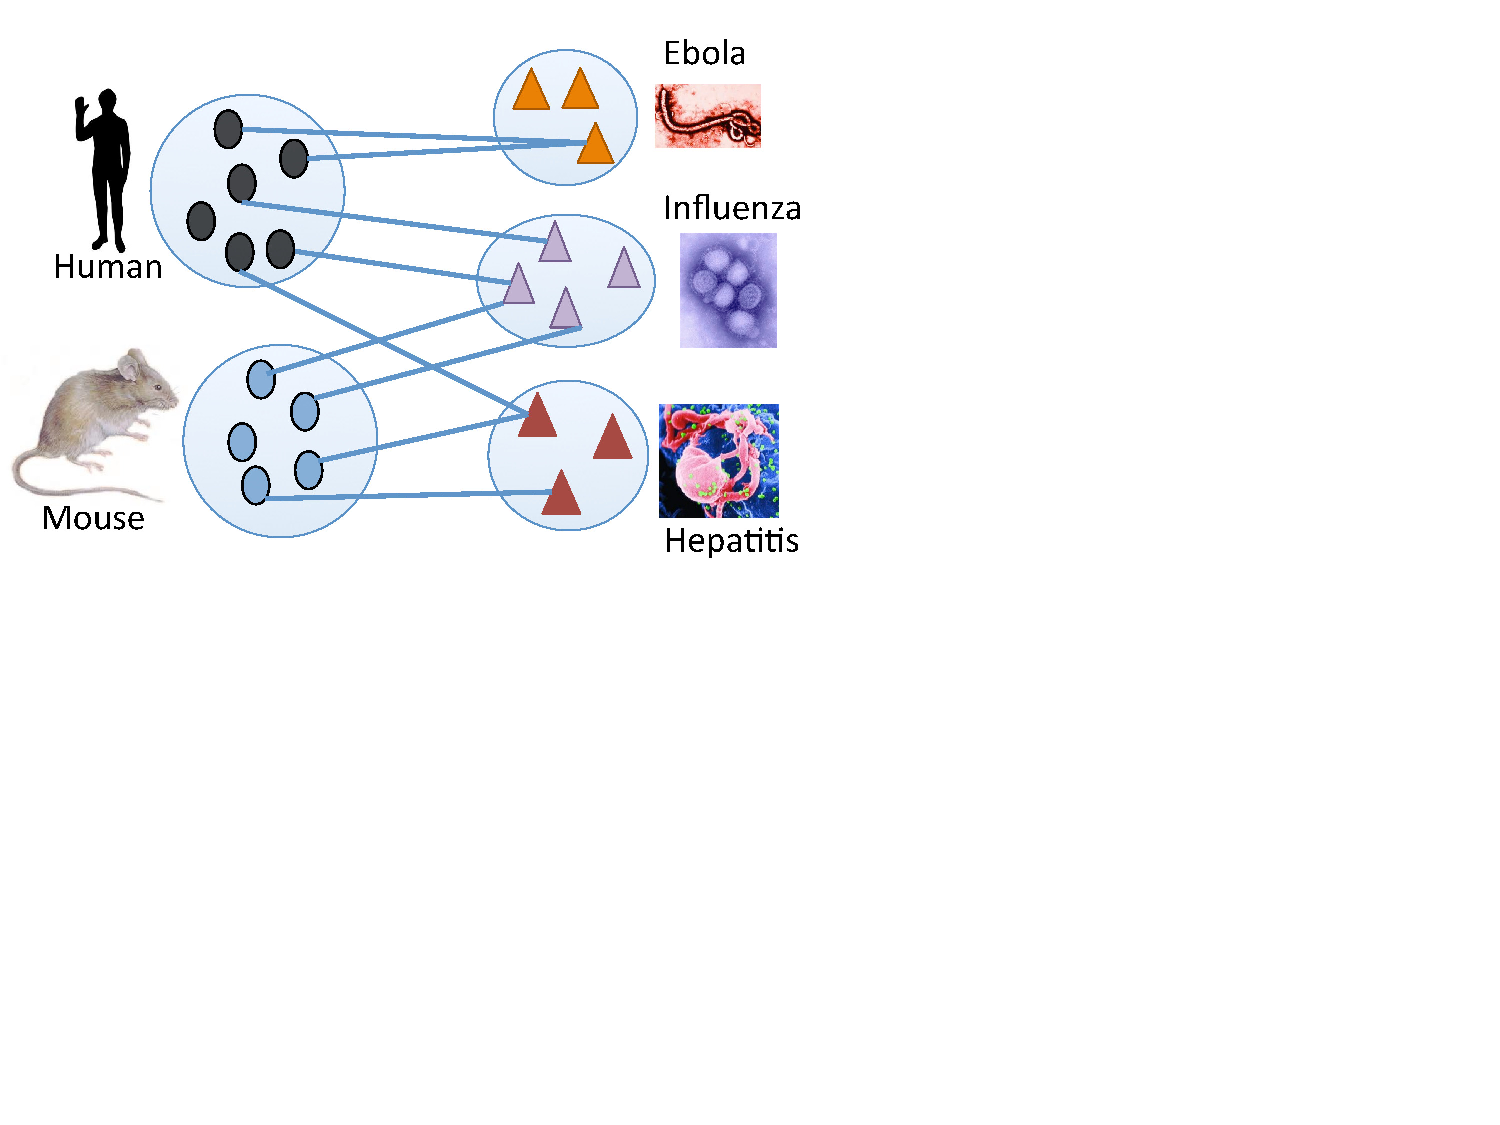
\includegraphics[scale=0.35, trim = 0.2 9.2cm 4cm 0]{fig1-eps-converted-to.pdf}
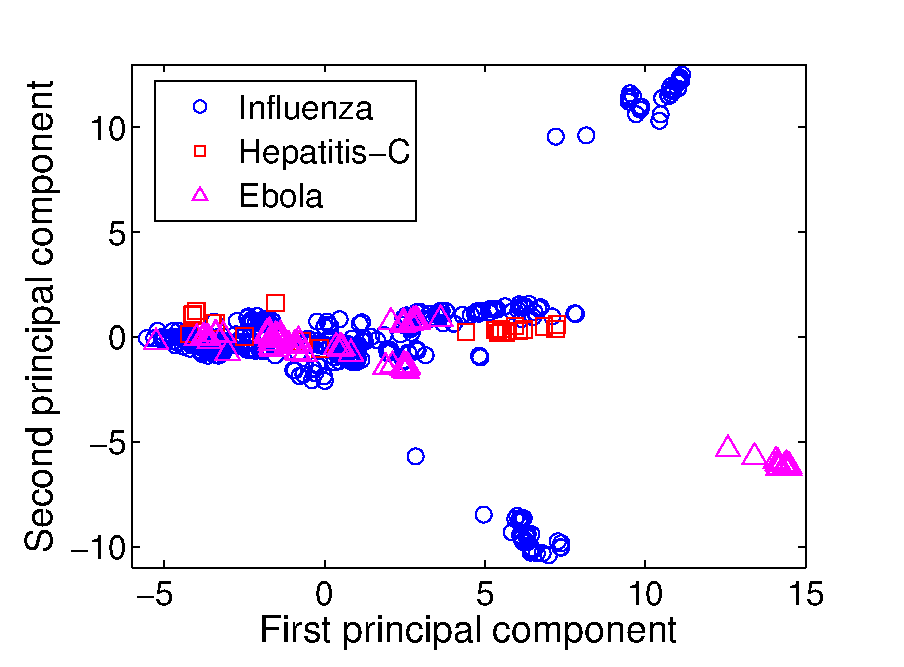
\includegraphics[scale=0.32, trim = 0 0 0 0]{pca_original_feats.eps}
}
{
\caption{Principal component analysis (PCA) of virus proteins in the original feature space. The first two principal components are shown. Shape and color of the points indicates which virus that protein comes from.}%
\label{fig:pca1}
%\caption{Multiple bipartite graphs: on the left are host proteins and on the right are proteins from different virus species. Edges represent protein interactions.}
%\label{fig:hpppigraph}
}
\end{floatrow}
\end{figure*}


\section{The bilinear sparse low-rank multitask model (BSL-MTL)} 
\label{ourmodel}
In the previous section, we described the bilinear low-rank model for matrix completion. 
Note that in order to capture linear functions over the features, we introduce a constant feature for every protein 
(i.e $[\mathbf{x}_i 1]$). We now discuss the multitask extensions that we propose. Let $\{\mathcal{G}_t\}$ where $t=1 \ldots T$ be the set of $T$ bipartite graphs and the corresponding matrices be $\{M_t\}$. Each matrix $M_t$ has rows corresponding to node type $\upsilon_t$ and columns corresponding to the node type $\varsigma_t$. The feature vectors for individual nodes of the two types be represented by $\mathbf{x}_{ti}$ and $\mathbf{y}_{tj}$ respectively. Let $\Omega_t$ be the set of observed links (and non-links) in the graph $\mathcal{G}_t$. Our goal is to learn individual link prediction functions $f_t$ for each graph. In order to exploit the relatedness of the $T$ bipartite graphs, we make some assumptions on how they share information. We assume that each matrix $M_t$ has a low-rank decomposition that is shared across all graphs and a sparse component that is specific to the task $t$. That is,
\begin{equation}
f_t(\mathbf{x}_{ti}, \mathbf{y}_{tj}) = \mathbf{x}_{ti}^\intercal H_t \mathbf{y}_{tj}, \textrm{ where } H_t = \mu_t U V^\intercal + (1-\mu_t)  S_t
\end{equation}

As before, the shared factors $U$ and $V$ are both $\mathbb{R}^{d_t \times k}$ (where the common dimensionality $d_t$ of the two node types is assumed for convenience). The matrix $S_t \in \mathbb{R}^{d_t \times d_t}$ is a sparse matrix. The objective function for the multitask model is given by:
\begin{equation}
\label{mtl_objective}
\begin{array}{ll}
\mathcal{L}(U,V,\{S_t\}) & = \displaystyle{ \frac{1}{N} \sum_{t=1}^T \sum_{(i,j) \in \Omega_t}} c^t_{ij} \; \ell \big( M_{t_{ij}}, \mathbf{x}_{ti}^\intercal H_t \mathbf{y}_{tj} \big) + \\
& \lambda ( \|U\|^2_F + \|V\|^2_F ) + \displaystyle{\sum_{t=1}^T \sigma_t \|S_t\|_1} 
\end{array}
\end{equation}

Here $N = \sum_t | \Omega_t |$, is the total number of training examples (links and non-links included) from all tasks. To enforce the sparsity of $S_t$ we apply an $\ell_1$ norm. In our experiments, we tried both $\ell_1$ and $\ell_2$ norms and found that the $\ell_1$ norm works better.


%\input{altmin_algo.tex}

\noindent \textbf{Optimization}:
The function $\mathcal{L}(U, V, \{S_t\})$ is non-convex. However, it is convex in every one of the parameters (i.e when the other parameters are fixed) 
and a block coordinate descent method called alternating least squares (ALS) is commonly used to optimize such functions. 
To speed up convergence we use an adaptive step size. The detailed optimization procedure is shown in the supplementary.
%Algorithm \ref{alg}. 

\noindent \textbf{Convergence:} The ALS algorithm is guaranteed to converge only to a local minimum. There is work showing convergence guarantees to global optima for related simpler problems, however the assumptions on the matrix and the parameter structure are not very practical and 
it is difficult to verify whether they hold for our setting. \\
\noindent \textbf{Initialization of $U$ and $V$}: We tried random initialization (where we randomly set the values to lie in the range [0 1]), and also 
the following strategies that initialize: $U^0 \leftarrow$ top-$k$ left singular vectors, and $V^0 \leftarrow$ top-$k$ right singular vectors from 
the SVD of $\displaystyle{\sum_{(i,j) \in \Gamma}} m_{ij} \mathbf{x}_i \mathbf{y}_j^\intercal$. We set $\Gamma$ to 
(a) training examples from all tasks, or (b) a random sample of 10000 unlabeled data from all tasks. We found that using the unlabeled data for initialization gives us a better performance.

%(a) \textit{Training data}: $\Gamma$ is set to all the training examples from all tasks. This initialization from Jain et al. \cite{prateek} uses the labels of the examples.\\
%(b) \textit{Unlabeled data}: $\Gamma$ is set to . Note that there are no labels $m_{ij}$ available here. In our experiments we found that using the unlabeled data for initialization gives us a better performance than using the training data or random initialization. 



\subsection{Handling the `curse of missing negatives'}
\label{negs}
For the MC algorithm to work in practice the matrix entries $M_{ij}$ should represent interaction scores (range [0 1]) 
or take binary values (1s for positives and 0s for negatives). Our experiments with PPI probabilities (obtained using the MINT-scoring algorithm)
gave bad models. The binary matrix setting requires some observed 0s. However non-interactions are not available as they cannot be verified 
experimentally for various reasons. Hence we derived a set of `probable negatives' using a heuristic often used in PPI prediction 
work \citep{qi06,qi09,dyer11,me_ismb_2013}. We pair up all virus proteins with all human proteins and sample a random set to be negatives. 
This heuristic works in practice as the interaction ratio (i.e number of positives in a large random set of protein pairs) is expected to be very low:
$\approx$ 1/100 to 1/500. That is, the probability that our negatives contain true positives is negligible. \\
\textbf{High class imbalance}: We incorporate the prior on the interaction ratio by setting the size of our randomly sampled negatives set equal to
100 times the number of gold standard positives.



\section{Dataset}
\label{sec:datasets}
We use three human-virus PPI datasets from the PHISTO \citep{phisto} database (version from 2014), the characteristics of which are summarized in Table \ref{datasets}. 
The \textit{Influenza A} task includes various strains of flu such as: H1N1 (Puerto Rico, Texas strains etc), H3N2 (England strain etc), H5N1, H7N3.
The \textit{Hepatitis} task has several subtypes (1a, 1b), isolates such as H77, HC-J6 etc and \textit{Ebola} has the Zaire ebolavirus strain Mayinga and strain 1995.
All three are single-strand RNA viruses, with \textit{Hepatitis} being a positive-strand ssRNA whereas \textit{Influenza} and \textit{Ebola} are negative-strand viruses. The density of the known interactions is quite small when considering the entire proteome (i.e all known proteins) of the host and pathogen species (last row in Table \ref{datasets}). \\

\subsection{Addressing the homologs in PHISTO}
\label{sec:phisto}
The interactions data reported in PHISTO database is aggregated from several host-pathogen interactions data sources such as MINT, IntAct, DIP etc. We found that many of the interactions (within a task) involve homologous PPI - virus protein homologs from two strains interacting with either the same human protein or with homologous human proteins. Such PPI usually come from different publications/ studies, but they introduce a lot of redundancy in the dataset. Removing such PPI is challenging as there are several criteria to consider, the most important being: \textit{what threshold of sequence similarity constitutes a homolog}? The very existence of sequence similarity between proteins is what makes it possible for biologists to predict unknown interactions and most computational methods rely on it for PPI prediction. 

In row-2 of Table \ref{datasets}, we give a conservative estimate of the number of non-homologous PPI. For this, we identify homologous PPI and retain only one of them in the dataset. Homologs were obtained using BLAST sequence alignment (blastp) using an e-value cut-off threshold of $1e^{-5}$. This is a relaxed cut-off since there are cases where two functionally different proteins (either virus-virus or human-human) with low query coverage and low identity end up as `homologs'. For example, human proteins Q8WV28 (gene BLNK, B-cell linker protein) and O00459 (gene PIK3R2, Phosphatidylinositol 3-kinase) are considered homologs by this cut-off. The number of non-homologous PPI should therefore be considered a lower limit.

In our experiments section, we thus evaluate our models in two settings - (1) on the original dataset (2) by creating partitions: the first without any homologous PPI and the other with only the homologous PPI.

%and thus interologs (within a task), the presence of which may not give a clear picture of a computational model. However these are reported by different publications/studies and were found using different experimental methods, so we do not exclude them and instead report performance on 

\subsection{Features}
Since the sequence of a protein determines its structure and consequently its function, it may be possible to predict PPIs using the amino acid sequence of a protein pair. \cite{shen:2007} introduced the ``conjoint triad model'' for predicting PPIs using only amino acid sequences. They partitioned the twenty amino acids into seven classes based on their electrostatic and water affinities.\footnote{For details of these classes, please refer to the supplementary or the original paper}
A protein's amino acid sequence is first transformed to a class-sequence (by replacing each amino acid by its class).
For $k$=3, they count the number of times each distinct tri-mer (set of three consecutive amino acids) occurred in the sequence.
Since there are 343 ($7^3$) possible tri-mers (with an alphabet of size 7), the feature vector containing the tri-mer frequency counts will have 343 elements.
To account for protein size, they normalized the counts by linearly transforming them to lie between 0 and 1.
Thus the value of each feature in the feature vector is the normalized count for each of the possible amino acid three-mers. We use di-, tri- and four-mers thus leading to a total of 2793 features ($7^2 + 7^3 + 7^4$).
Such features have been successfully applied in prior work \citep{dyer07,me_ismb_2013}.

\begin{figure*}
\begin{floatrow}
\capbtabbox[0.68\textwidth]{%
\begin{small}
\begin{center}
%\def\arraystretch{1.2}
\begin{tabular}{c|ccccccc}
\toprule
& \multicolumn{3}{c}{\textbf{10\% training, 90\% test}} && \multicolumn{3}{c}{\textbf{30\% training, 70\% test}} \\ \cline{2-4}\cline{6-8}
& \textit{Ebola} & \textit{Hep-C} & \textit{Influenza} && \textit{Ebola} & \textit{Hep-C} & \textit{Influenza} \\ \midrule
Homolog & \textbf{0.230}$\pm$.06 & 0.178$\pm$.01 & 0.158$\pm$.01 && \textbf{0.311}$\pm$.03 & 0.180$\pm$.01 & 0.198$\pm$.01 \\
STL (Ridge Reg.)  & 0.189$\pm$.09 & 0.702$\pm$.08 & 0.286$\pm$.02 && 0.130$\pm$.03 & 0.802$\pm$.03 & 0.428$\pm$.03 \\ 
MMTL & 0.113$\pm$.04 & 0.767$\pm$.03 & 0.321$\pm$.02 && 0.129$\pm$.02 & 0.802$\pm$.04 & 0.430$\pm$.03  \\ 
%Trace-norm  & 0.199$\pm$.11 & 0.767$\pm$.03 & 0.318$\pm$.02 && 0.207$\pm$.02 & 0.808$\pm$.02 & 0.409$\pm$.03 \\ 
Sparse+low-rank & 0.144$\pm$.07 & 0.767$\pm$.02 & 0.318$\pm$.02 && 0.153$\pm$.02 & \textbf{0.814}$\pm$.01 & 0.414$\pm$.03  \\ 
%Dirty model \citep{jalali2010} & 0.074$\pm$.03 & 0.767$\pm$.04 & 0.324$\pm$.02 && 0.165$\pm$.02 & 0.813$\pm$.03 & 0.412$\pm$.03  \\ 
MTPL & 0.217$\pm$.08 & 0.695$\pm$.02 & 0.345$\pm$.02 && 0.260$\pm$.05 & 0.713$\pm$.01 & \textbf{0.496}$\pm$.03 \\ 
IMC & 0.087$\pm$.04 & \textbf{0.779}$\pm$.02 & \textbf{0.362}$\pm$.01 && 0.122$\pm$.02 & 0.801$\pm$.01 & 0.410$\pm$.03  \\ \midrule
BSL-MTL & \textbf{0.233}$\pm$.10 & \textbf{0.807}$\pm$.02 & \textbf{0.486}$\pm$.02 && \textbf{0.361}$\pm$.03 & \textbf{0.842}$\pm$.01 & \textbf{0.560}$\pm$.02  \\ \bottomrule
\end{tabular}
\end{center}
\end{small}
}
{
\caption{Area Under the Precision-Recall curve (AUC-PR) on the PHISTO dataset. The column header `X\% training' indicates the fraction of the labeled data used for training and tuning the model with the rest (100-X)\% used as test data. We report the average AUC-PR over 10 random train-test splits (stratified splits that maintain the class-skew of 1:100). The standard deviation is also shown. The performance of the best baseline and the overall best method (BSL-MTL) is highlighted in bold. The Homolog baseline performs comparably to our BSL-MTL method on the \textit{Ebola} task. This is explained by the virus-human PPI graph, from several other viruses, that the Homolog baseline has access to.}
\label{resultsTable}
}

\ffigbox[0.28\textwidth]{%
%%trim option's parameter order: left bottom right top
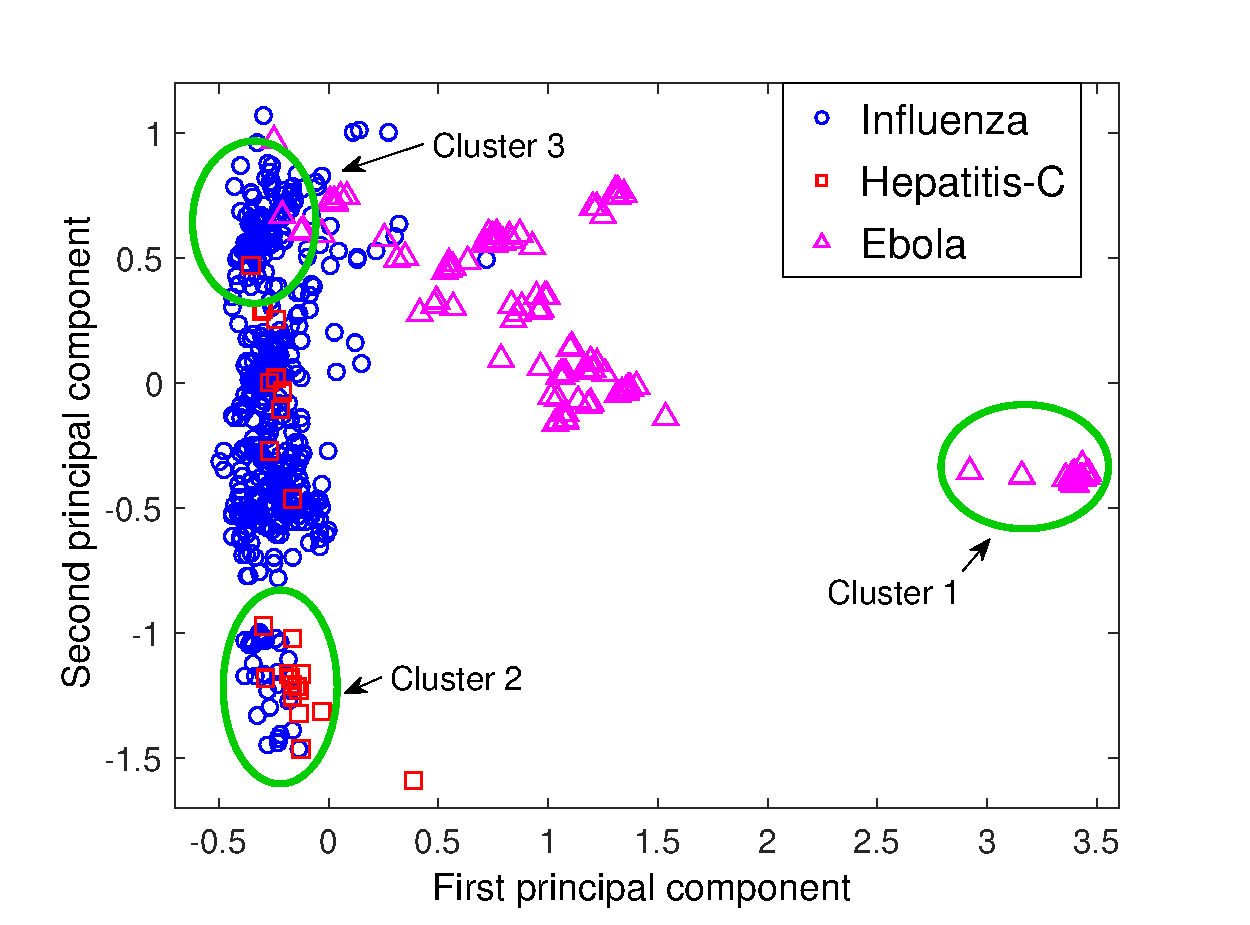
\includegraphics[scale=0.28, trim = 0.8cm 0.5cm 0 0]{pca_bslmtl_with_clusters.eps}
}
{
\caption{Principal component analysis (PCA) of virus proteins in the projected subspace. The first two principal components are shown. Shape of the points indicates which virus that protein comes from. We have highlighted three clusters for which we show GO term enrichment analysis results in Table \ref{goterms}.}%
\label{fig:pca2}
}
\end{floatrow}
\end{figure*}





\section{Experimental setup}

\subsection{Comparison with other machine learning approaches}
\label{mlmethods}
Our baselines include recent low-rank and sparse models, conventional multitask methods and prior work on HP PPI prediction. For a uniform comparison we used least squared loss in all the methods. The MALSAR \citep{malsar} package was used to implement some of the models. For the baselines wherever appropriate, we concatenated the features of the two node types into a single feature vector. Let $W \in \mathbb{R}^{T \times d_t}$ be the matrix with the task-specific weight vectors $\mathbf{w}_t$.
 
\noindent\textbf{Single task (STL)}: We used ridge regression with $\ell_2$ regularization (which performed better than $\ell_1$). \\
\noindent\textbf{MMTL}: The mean regularized multitask learning model from \cite{pontil04}. \\
\noindent\textbf{Sparse + low-rank} \citep{chen2012}: $W$ is assumed to have the decomposition: $W = P + Q$, where $P$ is sparse and $Q$ has a low-rank structure. \\
\noindent\textbf{IMC} \citep{prateek,nagarajan}: This is the link-prediction model from Section \ref{MCintro}, where data from all tasks is combined without incorporating any task relationships. $U$ and $V$ are shared by all tasks. We use the same initialization for this method as we do for our model. A comparison to this model tells us how much we gain from the task-specific sparsity component $S_t$. \\
\noindent\textbf{MTPL} \citep{me_ismb_2013}: A biologically inspired regularizer is used to capture task similarity.\\ \noindent\textbf{BSL-MTL}: Bilinear sparse low-rank multitask learning, the method developed in this paper.



\subsection{Comparison with a homolog baseline}
In addition to the machine learning methods presented in Section \ref{mlmethods}, we also tried a simple homology based approach.
As per this method, a virus protein $v$ will interact with a human protein $h$ if it interacts with any other human protein $h'$ similar to $h$. The converse holds too. Such homology-motivated heuristic approaches have been traditionally popular in the inter-organism PPI prediction literature \citep{vidal:2001,matthews:2001}. \cite{mika:2006} offers a commentary on the the success of such approaches in prediction PPI within an organism and the transferability across organisms. Modifications of such approaches have been published recently \citep{chen:2009,lin:2013,murakami:2014}.

The virus-virus and human-human protein similarity graphs used in this baseline were computed using protein sequence similarity.
We ran BLAST sequence alignment (\texttt{blastp}) with an e-value cut-off of 0.1 and the negative logarithm of the e-value was used as a measure of similarity (we use a somewhat relaxed cut-off as we are comparing across organisms).
We use the entire human-virus interactome from PHISTO as input to this method. Given a human protein $h$, we rank all virus proteins $v$ based on the following simple scheme. Let $V(h)$ be a set of all virus proteins interacting with the human protein $h$ and let $H(v)$ be all human proteins interacting with the virus protein $v$. We score each pair $(h, v)$ from the bipartite graph as follows: $\max \{ \max $ similarity between $h$ and all human proteins in $H(v)$; $\max $ similarity between $v$ and all virus proteins in $V(h) \}$. 
This baseline is shown in the first row as \textit{Homolog} in Table \ref{resultsTable}.


\subsection{Evaluation setup}
We compare all the methods in two settings, where a small proportion of the available labeled data is randomly sampled and used to train a model which is then evaluated on the remaining data. For the first setting we randomly split the labeled data from each task into 10\% training and 90\% test, such that the class-skew of 1:100 is maintained in both splits (i.e stratified splits). The second setting uses a 30\% training, 70\% test split. 
In each setting we generate ten random splits and average the performance over the ten runs (parameter tuning details are in the supplementary).

We report the area under the precision recall curve (AUC-PR) along with the standard deviation. 
AUC-PR has been shown to give a more informative picture of an algorithm's performance than ROC curves in high class imbalance datasets \citep{davis2006} such as ours. 

%Cold-start: The test data can contain edges over nodes that were never seen during training. The number of such unseen nodes in the test data, on an average was: in the \textit{10\%} setting: 536.4 unseen nodes and in \textit{30\%}: ????? new nodes in test data.



\section{Results}
The PPI data we obtain from PHISTO has homologous PPI within a task. Note that the presence of sequence similarity across virus proteins is a strong criterion for computational methods to work, however orthologs or paralogs of proteins within a task lead to redundancy in the data and some readers may find it harder to judge the contribution of the methods. We therefore present results on three sets: 
\begin{enumerate}[a]
\item the original PPIs from PHISTO. AUC-PR is shown in Table \ref{resultsTable}
\item \textbf{Non-homologous partition}: after removal of all homologous PPI from the test data. Here we ensure that the test data does not contain homologs of PPI observed in the training data (this ensures there are no redundant examples). Further, every set of homologous PPIs in the test data is replaced with a single PPI. A BLAST sequence similarity cut-off of $1e^{-5}$ was used to find homologs. The results are in Table \ref{nohomresultsTable}.
\item \textbf{Homologous PPI partition} : only homologous PPI part of the test data. This is essentially the set of PPI removed in the set-(b) above. Table \ref{homresultsTable} shows these results. 
\end{enumerate}
Note that the partitions in (b) and (c) together comprise our test data. Also, the negatives in the test data are randomly split into the `no-homolog' and 'homolog' partitions while maintaining the number of negatives in each partition to be 100 times the number of positives. 

\noindent\textit{Overall performance}
For reference, the AUC-PR of a random classifier model is $\approx 0.01$ due to the class imbalanced nature of the data.
In general, we notice that multitask learning benefits
all tasks. The first three columns show the results in the 10\% setting. 
%The number of training positive examples from each task are 8 for Ebola, 85 for Influenza and 98 for Hepatitis-C. 
Our model (last row) has large gains for Influenza (1.4 times better than the next best) and modest improvements for the other tasks.
The variance in the AUC is high for the Ebola task (column 1) owing to the small number of positives 
in the training splits.
The most benefits for our model are seen in the 30\% setting for all tasks.
Notably, Homolog performs comparably to our model. In addition to the training data seen by all other methods, this baseline also uses additional data in the form of the virus-virus, human-human sequence similarities and a virus-human interactome from several other viruses (besides the three tasks). 
Results on the partitions shed further light on this.

\noindent\textit{Performance on the non-homologous PPI partition}:
Table \ref{nohomresultsTable} has these results. Overall, our method performs best on this partition over all tasks.
Comparison with the AUC in Table \ref{resultsTable} shows that AUC for the \textit{Ebola} task is higher on all baselines except Homolog, indicating that
a bigger fraction of the overall performance comes from the non-homologous partition (this is also marginally the case for \textit{Influenza}). 
This effect is the most pronounced for our method (BSL-MTL)
and demonstrates that we are able to predict such PPI by sharing information with other tasks. 
There are thus two components to the prediction performance - (1) the presence of sequence-similar proteins within a task (2) non-linear similarities between the interactions within a task and across tasks. We are able to capture the latter well via the shared subspace structure of our model.


%Homolog & 0.010 $\pm$.03 & 0.079 $\pm$.01 & 0.135 $\pm$.02 \\  
%STL (Ridge Reg.)  & 0.054 $\pm$.03 &  0.400 $\pm$.06 & 0.192 $\pm$.03 \\
%BSL-MTL (this work) & 0.071 $\pm$.03 & \textbf{0.501} $\pm$.05 & \textbf{0.331} $\pm$.03  \\ \bottomrule 

\begin{table}[!h]
\caption{AUC-PR on the \textbf{non-homologous PPI within each task}, in the 10\% setting. To get an estimate of the relative size of the non-homologous partition for each task, see Table \ref{datasets}. Only the most representative baselines are retained for this experiment. Our model performs better than the others on the non-homologous part of the test data, as it captures non-linear similarities among the interactions within a task and across tasks very well.}
\label{nohomresultsTable}
\begin{small}
\begin{center}
%\def\arraystretch{1.2}
\begin{tabular}{c|ccc}
\toprule
\multicolumn{4}{c}{\textbf{10 \% training, 90\% test on Non-homologous PPI}} \\
& \textit{Ebola} & \textit{Hep-C} & \textit{Influenza} \\ \midrule
Homolog & 0.207 $\pm$.07 & 0.113 $\pm$.01 & 0.109 $\pm$ .01 \\
STL  & 0.210 $\pm$.14 & 0.474 $\pm$ .06 & 0.302 $\pm$.03 \\
Sparse+LR & 0.216 $\pm$.13 & 0.482 $\pm$.05 & 0.312 $\pm$.04 \\ 
BSL-MTL & \textbf{0.295} $\pm$.10 & \textbf{0.544} $\pm$.06 & \textbf{0.505} $\pm$.05 \\ \bottomrule
\end{tabular}
\end{center}
\end{small}
\end{table}


\noindent\textit{Performance on the homologous PPI partition} (Table \ref{homresultsTable}):
Except the \textit{Ebola} task, BSL-MTL has the highest AUC. The Homolog baseline best captures the homologous PPI in \textit{Ebola} (with an AUC twice the next best). However, since there are far fewer homologous PPI in Ebola than in the other tasks (row-2 of Table \ref{datasets}), this contributes less to the overall performance of the Homolog baseline. \textit{Hepatitis-C} has the highest fraction of homologous PPI and BSL-MTL does significantly better on these than the other baselines which also leads to a higher overall AUC. The same can be said of the \textit{Influenza} task.

%\subsection{Disadvantages of the Homolog method}
%In Figure \ref{fig:network} we show for each task, the protein interactions in the test data (for one train-test split) that were not found by the homologs model which relies purely on homology-based sequence similarity. The interactions mainly involve human proteins which do not have a homolog in the training data. This illustrates that our features capture more information than mere sequence similarity. Further, inclusion of interactions from other viruses in the na\"ive manner as done by the homologs in fact hurts the performance (results in too many false positives) - our model is able to learn what to borrow from the other tasks accurately.

\begin{table}[!h]
\caption{AUC-PR on the \textbf{homologous PPI} within each task, in the 10\% setting. The Homolog baseline outperforms all on the \textit{Ebola} task and BSL-MTL beats all other methods on the other tasks. The Homolog method has access to a wider virus-human PPI graph involving several other viruses and is able to infer homologous PPI for \textit{Ebola} better (note that some of the homologous PPI are not redundant examples but involve proteins with very small regions of sequence similarity.}
\label{homresultsTable}
\begin{small}
\begin{center}
%\def\arraystretch{1.2}
\begin{tabular}{c|ccc}
\toprule
\multicolumn{4}{c}{\textbf{10 \% training, test only Homologous PPI }} \\
& \textit{Ebola} & \textit{Hep-C} & \textit{Influenza} \\ \midrule
Homolog & \textbf{0.399} $\pm$.07 & 0.161 $\pm$.01 & 0.180 $\pm$ .01 \\
STL   & 0.192 $\pm$.15 & 0.504 $\pm$.10 & 0.305 $\pm$.03 \\
Sparse+LR & 0.184 $\pm$.13 & 0.512 $\pm$.10 & 0.315 $\pm$.04 \\ 
BSL-MTL & 0.130 $\pm$.10 & \textbf{0.815} $\pm$.02 & \textbf{0.475} $\pm$.02 \\ \bottomrule
\end{tabular}
\end{center}
\end{small}
\end{table}


\subsection{Biological significance of the model}
\label{bioanalysis}
The model parameters $U$, $V$ and $S$ are a source of rich information which can be used to further understand host-pathogen
interactions. Note that our features are derived from the amino acid sequences of the proteins which provide
opportunities to interpret the parameters.

\subsubsection{Clustering proteins based on interaction propensities}
We analyze the proteins by projecting them using the model parameters $U$ and $V$ into a lower dimensional subspace 
(i.e computing $X U^\intercal$ and $Y V^\intercal$ to get projections of the virus and human proteins respectively).  
The principal component analysis (PCA) of this lower dimensional representation is compared with PCA in the original feature space (protein sequence features) in Figures \ref{fig:pca1} and \ref{fig:pca2}. 
Firstly, the projected data has a much better separation than the original data.
Secondly, Fig \ref{fig:pca2} tells us that Hepatitis-C and Influenza have many proteins with similar binding tendencies, and that these behave differently than most Ebola virus proteins. This observation is not obvious in the PCA of the original feature space (Fig \ref{fig:pca1}), where proteins with similar sequences group together.
We analyze the projected data further by looking at the clusters of proteins for enrichment of Gene Ontology (GO) annotations (proteins were first clustered in this lower dimensional space using k-means and setting the number of clusters to 6). Of particular interest are the highlighted three clusters which contain either proteins projected far from others (such as cluster-1) and proteins from different viruses projected close together (cluster-2 and cluster-3).
For enrichment analysis, we use the FuncAssociate 3.0 \citep{funcAsso} tool and GO annotations for the three viruses from UniProtKB.


%\begin{figure}
%\begin{tabular}{c}
%%\begin{minipage}{0.3\textwidth}
%%\begin{center}
%%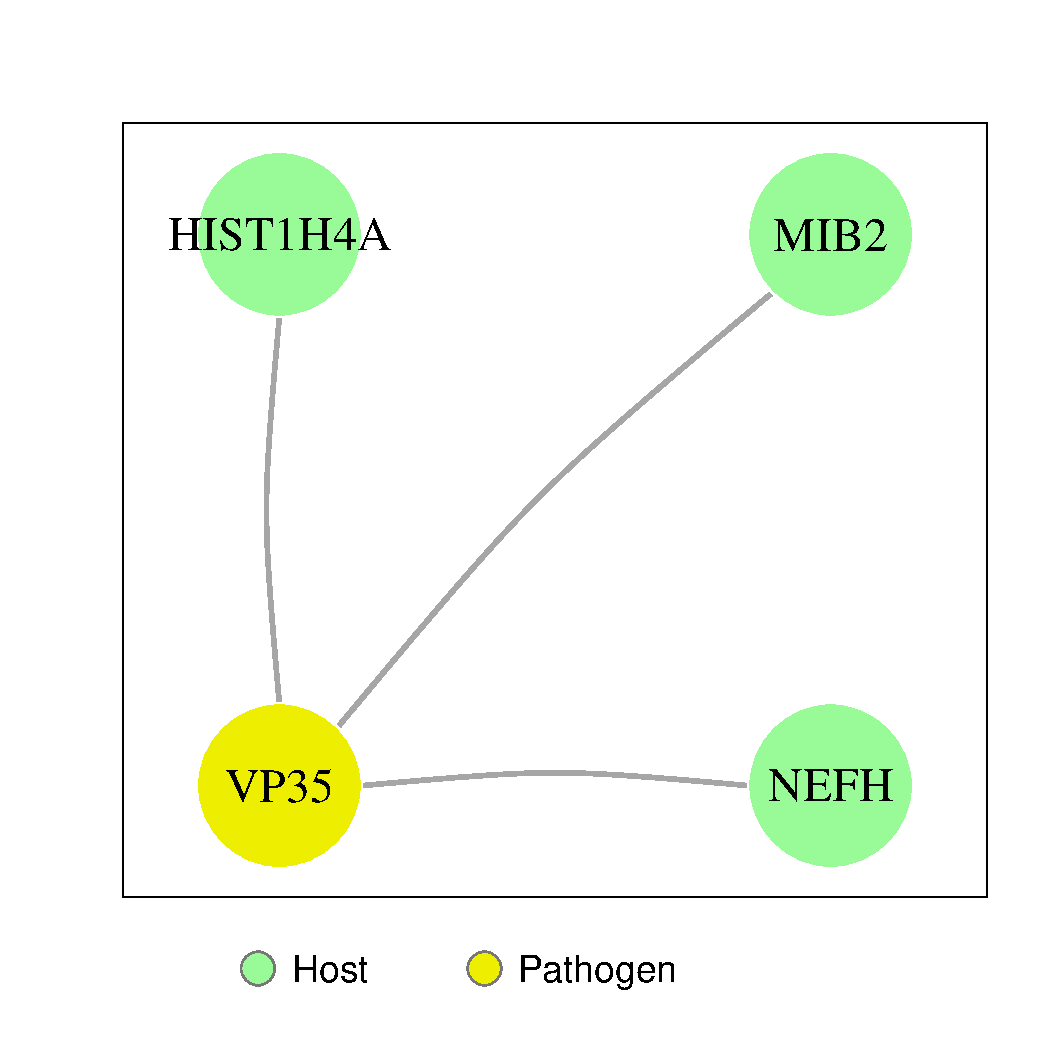
\includegraphics[scale=0.23, trim = 0.3 0 0.2 0.2]{ebolanet.pdf}\vspace{0.6cm}
%%\end{center}
%%\end{minipage}
%%&
%\begin{minipage}{\textwidth}
%\begin{center}
%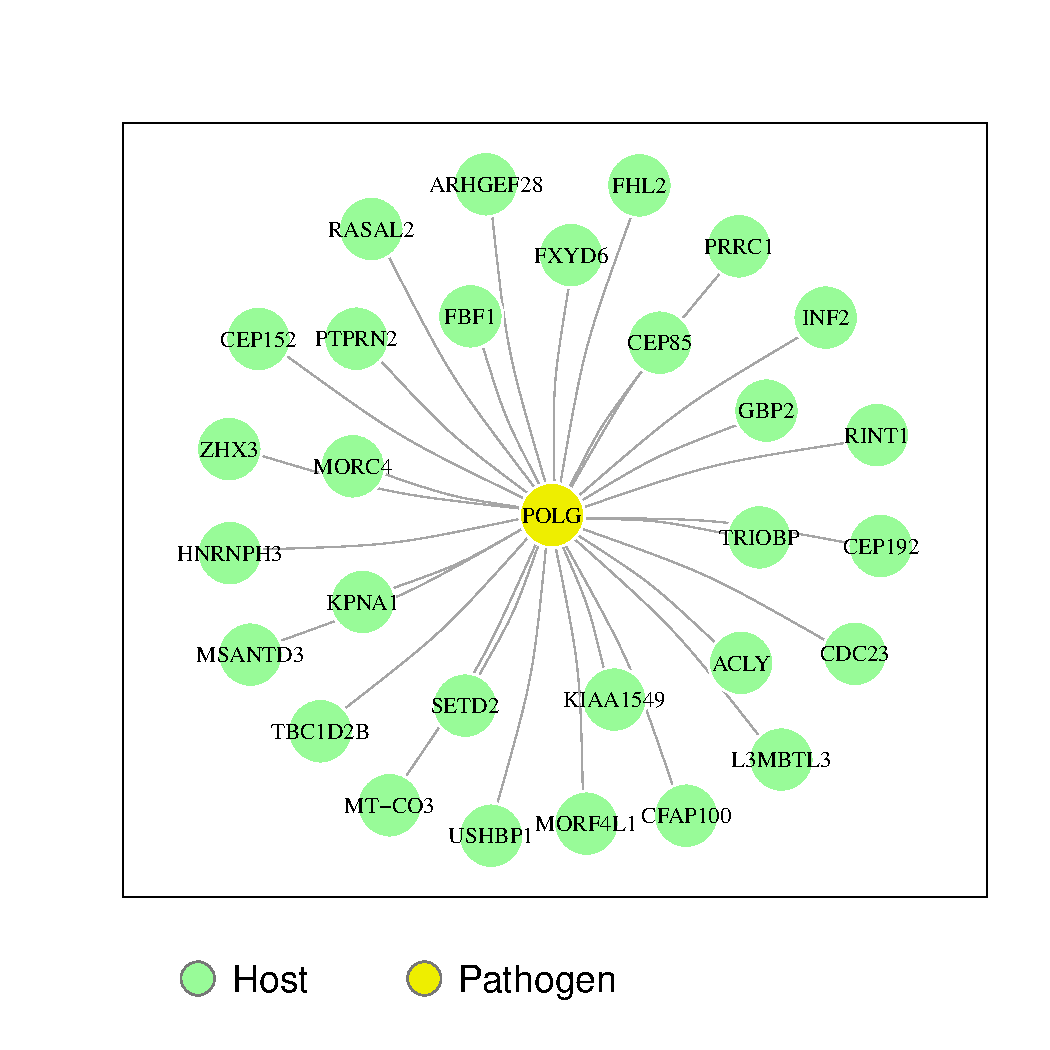
\includegraphics[scale=0.25, trim = 0.7cm 0.7cm 0.7cm 0.7cm]{flavinet.pdf}
%\end{center}
%\end{minipage}
%\\
%\begin{minipage}{\textwidth}
%\begin{center}
%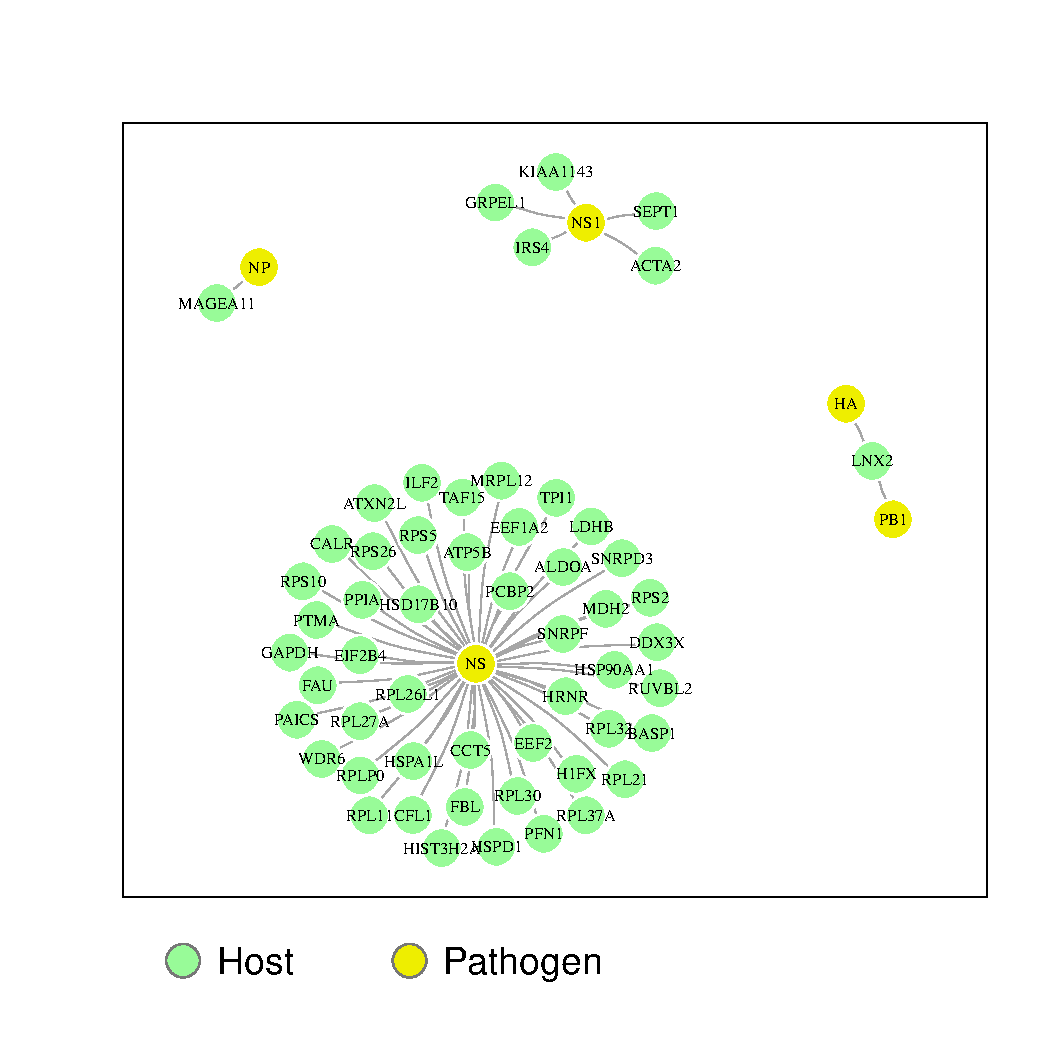
\includegraphics[scale=0.25, trim = 0.5cm 0.5cm 0.5cm 0.5cm]{flunet.pdf}
%\end{center}
%\end{minipage}
%\end{tabular}
%\caption{PPI from each task that are found by our method but are missed by the homolog method. To obtain these, we chose a random train/test split and picked examples from the test data on which the homolog method fails - these are ones for which sequence-similar proteins are not found. (a) shows \textit{Ebola}-human PPI, (b) \textit{Hepatitis-C} human PPI and (c) \textit{Influenza}-human PPI.}
%\label{fig:network}
%\end{figure}


\begin{table}[bht]
\begin{scriptsize}
\begin{center}
%\def\arraystretch{1.1}
\begin{tabular}{|c|c|}
\multicolumn{2}{c}{Gene Ontology terms for clusters from Figure \ref{fig:pca2}} \\ \hline
cluster 1 & mRNA (guanine-N7-)-methyltransferase activity; RNA-directed \\
(ebola only)& RNA polymerase activity; ATP binding \\ \hline
cluster 2 & host cell endoplasmic reticulum membrane; \\ 
(hepatitis \& & host cell lipid particle; induction by virus \\
influenza & of host autophagy; host cell mitochondrial membrane; \\
proteins) & suppression by virus of host STAT1 activity \\ \hline
cluster 3 (all) & fusion of virus membrane with host plasma membrane \\ \hline
\end{tabular}
\caption{GO terms (for process, function, component) enriched in the highlighted clusters from Figure \ref{fig:pca2}. FuncAssociate GO enrichment tool was used and terms with p-value < 0.001 are shown. The first column also indicates the composition of each cluster (i.e which task's proteins appear in the cluster).}
\label{goterms}
\end{center}
\end{scriptsize}
\end{table}

 


\subsubsection{Novel interactions with Ebola proteins}
%The correlations captured by $U V^\intercal$ and $S_t$ tell us which amino-acid $k$-mer pairs (one kmer from the host protein, one kmer from the pathogen protein) are important for interactions. Using these we can derive details of the putative protein interaction interfaces (i.e which parts of the molecules are in contact when the two proteins bind to each other). 
The top four Ebola-human PPI are all predictions for the Ebola envelope glycoprotein (GP) with four different human proteins (Note: GP is not in the gold standard PPIs). There is abundant evidence in the published literature \citep{nanbo2010} for the critical role played by GP in virus docking and fusion with the host cell.

%Our model not only provides predictions on whether or not two proteins interact, but can also provide hypotheses 
%as to the putative binding sites for the interaction. This is of significance for the viruses (esp. Ebola) as they have 
%very few proteins with known 3D structures. Traditional linear models do not give us correlations between amino acid residues. 
%We selected the top 10 Ebola-human PPI predictions (the novel interactions) from our model and analyzed their 3D structures (using the available structures in PDB). 
%For each predicted PPI we performed protein-protein docking using the ClusPro algorithm. 
%The sites that are within 10 the docking model also corresponded to the host-pathogen feature pairs 
%that were responsible for that particular prediction. The 3D structure of one predicted interaction and it's binding interface is shown in Figure \ref{fig:3dstructure}. 


%\begin{figure}[h]
%\caption{3D structure obtained by docking ebola virion spike glycoprotein (green) with human ubiquitin-protein ligase (cyan). The putative binding sites are shown using sticks.}%
%\label{fig:3dstructure}
%%trim option's parameter order: left bottom right top
%\includegraphics[scale=0.3, trim = 0 0.8cm 0 0]{images/interaction_3d_structure.png}
%\end{figure}

%%%%%%%%%%%%%%%%%%%%%%%%%%%%%%%%%




\subsubsection{Sequence motifs from virus proteins}
We analyze sequence motifs derived from the top $k$-mers that contribute to interactions. The significant entries of the model parameters $U$, $V$ and $\{S_t\}$ were used to 
compute these motifs. The top positive-valued entries from the product $U V^T$ indicate which pairs of features: ($(f_v, f_h)$: virus protein feature, human protein feature) are important for interactions across all the virus-human PPI tasks.
Analogously, the entries from $S_t$ give us pairs of features important to a particular virus-human task `$t$'.
These results are in the supplementary.\\


\noindent\textbf{Results on HIV data}: 
We incorporate an additional task: HIV (human immunodeficiency virus), which is quite dissimilar to our original setting involving three viruses (HIV is a retrovirus). This experiment tests how our multitask model behaves in the presence of a relatively outlier task. The interactions data has $\approx$4000 human-HIV PPI across several strains of which 1320 are non-homologous PPI. Please refer to the supplementary for the results.

\section{Conclusions and future extensions}
%Multitask link prediction is an important area with many applications ranging from recommendation systems to biomedical host-pathogen interactions.  
This work developed and tested a new multitask learning method for host-pathogen PPI prediction based on low-rank matrix completion for sharing information across tasks. Our method, BSL-MTL exhibited large increases in prediction accuracy compared to a variety of baselines.
%and showed significant increases in prediction performance. 
%The method was evaluated on host-pathogen protein interaction domain for three pathogens (three tasks) and exhibited large increases in prediction accurac
The model parameters provide several avenues for further studying host-pathogen PPI that can lead to interesting observations and insights. Finally, the model we present is general enough to be applicable on other problems such as: gene-disease relevance prediction across organisms or disease conditions. 


%%%%%%%%%%%%%%%%%%%%%%%%%%%%%%%%%

%\section*{Acknowledgement}

%\paragraph{Funding\textcolon} 

%\input{appendix.tex}


\bibliographystyle{natbib}
\begin{scriptsize}
\bibliography{references}
\end{scriptsize}

\end{document}
